\section{Robotics \& Non-Rigid Objects}
\frame{
  \frametitle{An Adaptive Robotic System for Doing Pick and Place Operations with Deformable Objects}
  Troels Bo Jørgensen, Sebastian Nesgaard Jensen, Henrik Aanæs, Niels Worsøe Hansen and Nobert Krüger

  \textit{Robotics and Computer-Integrated Manufacturing (Under review, Accepted)}
  \begin{figure}
    \centering
    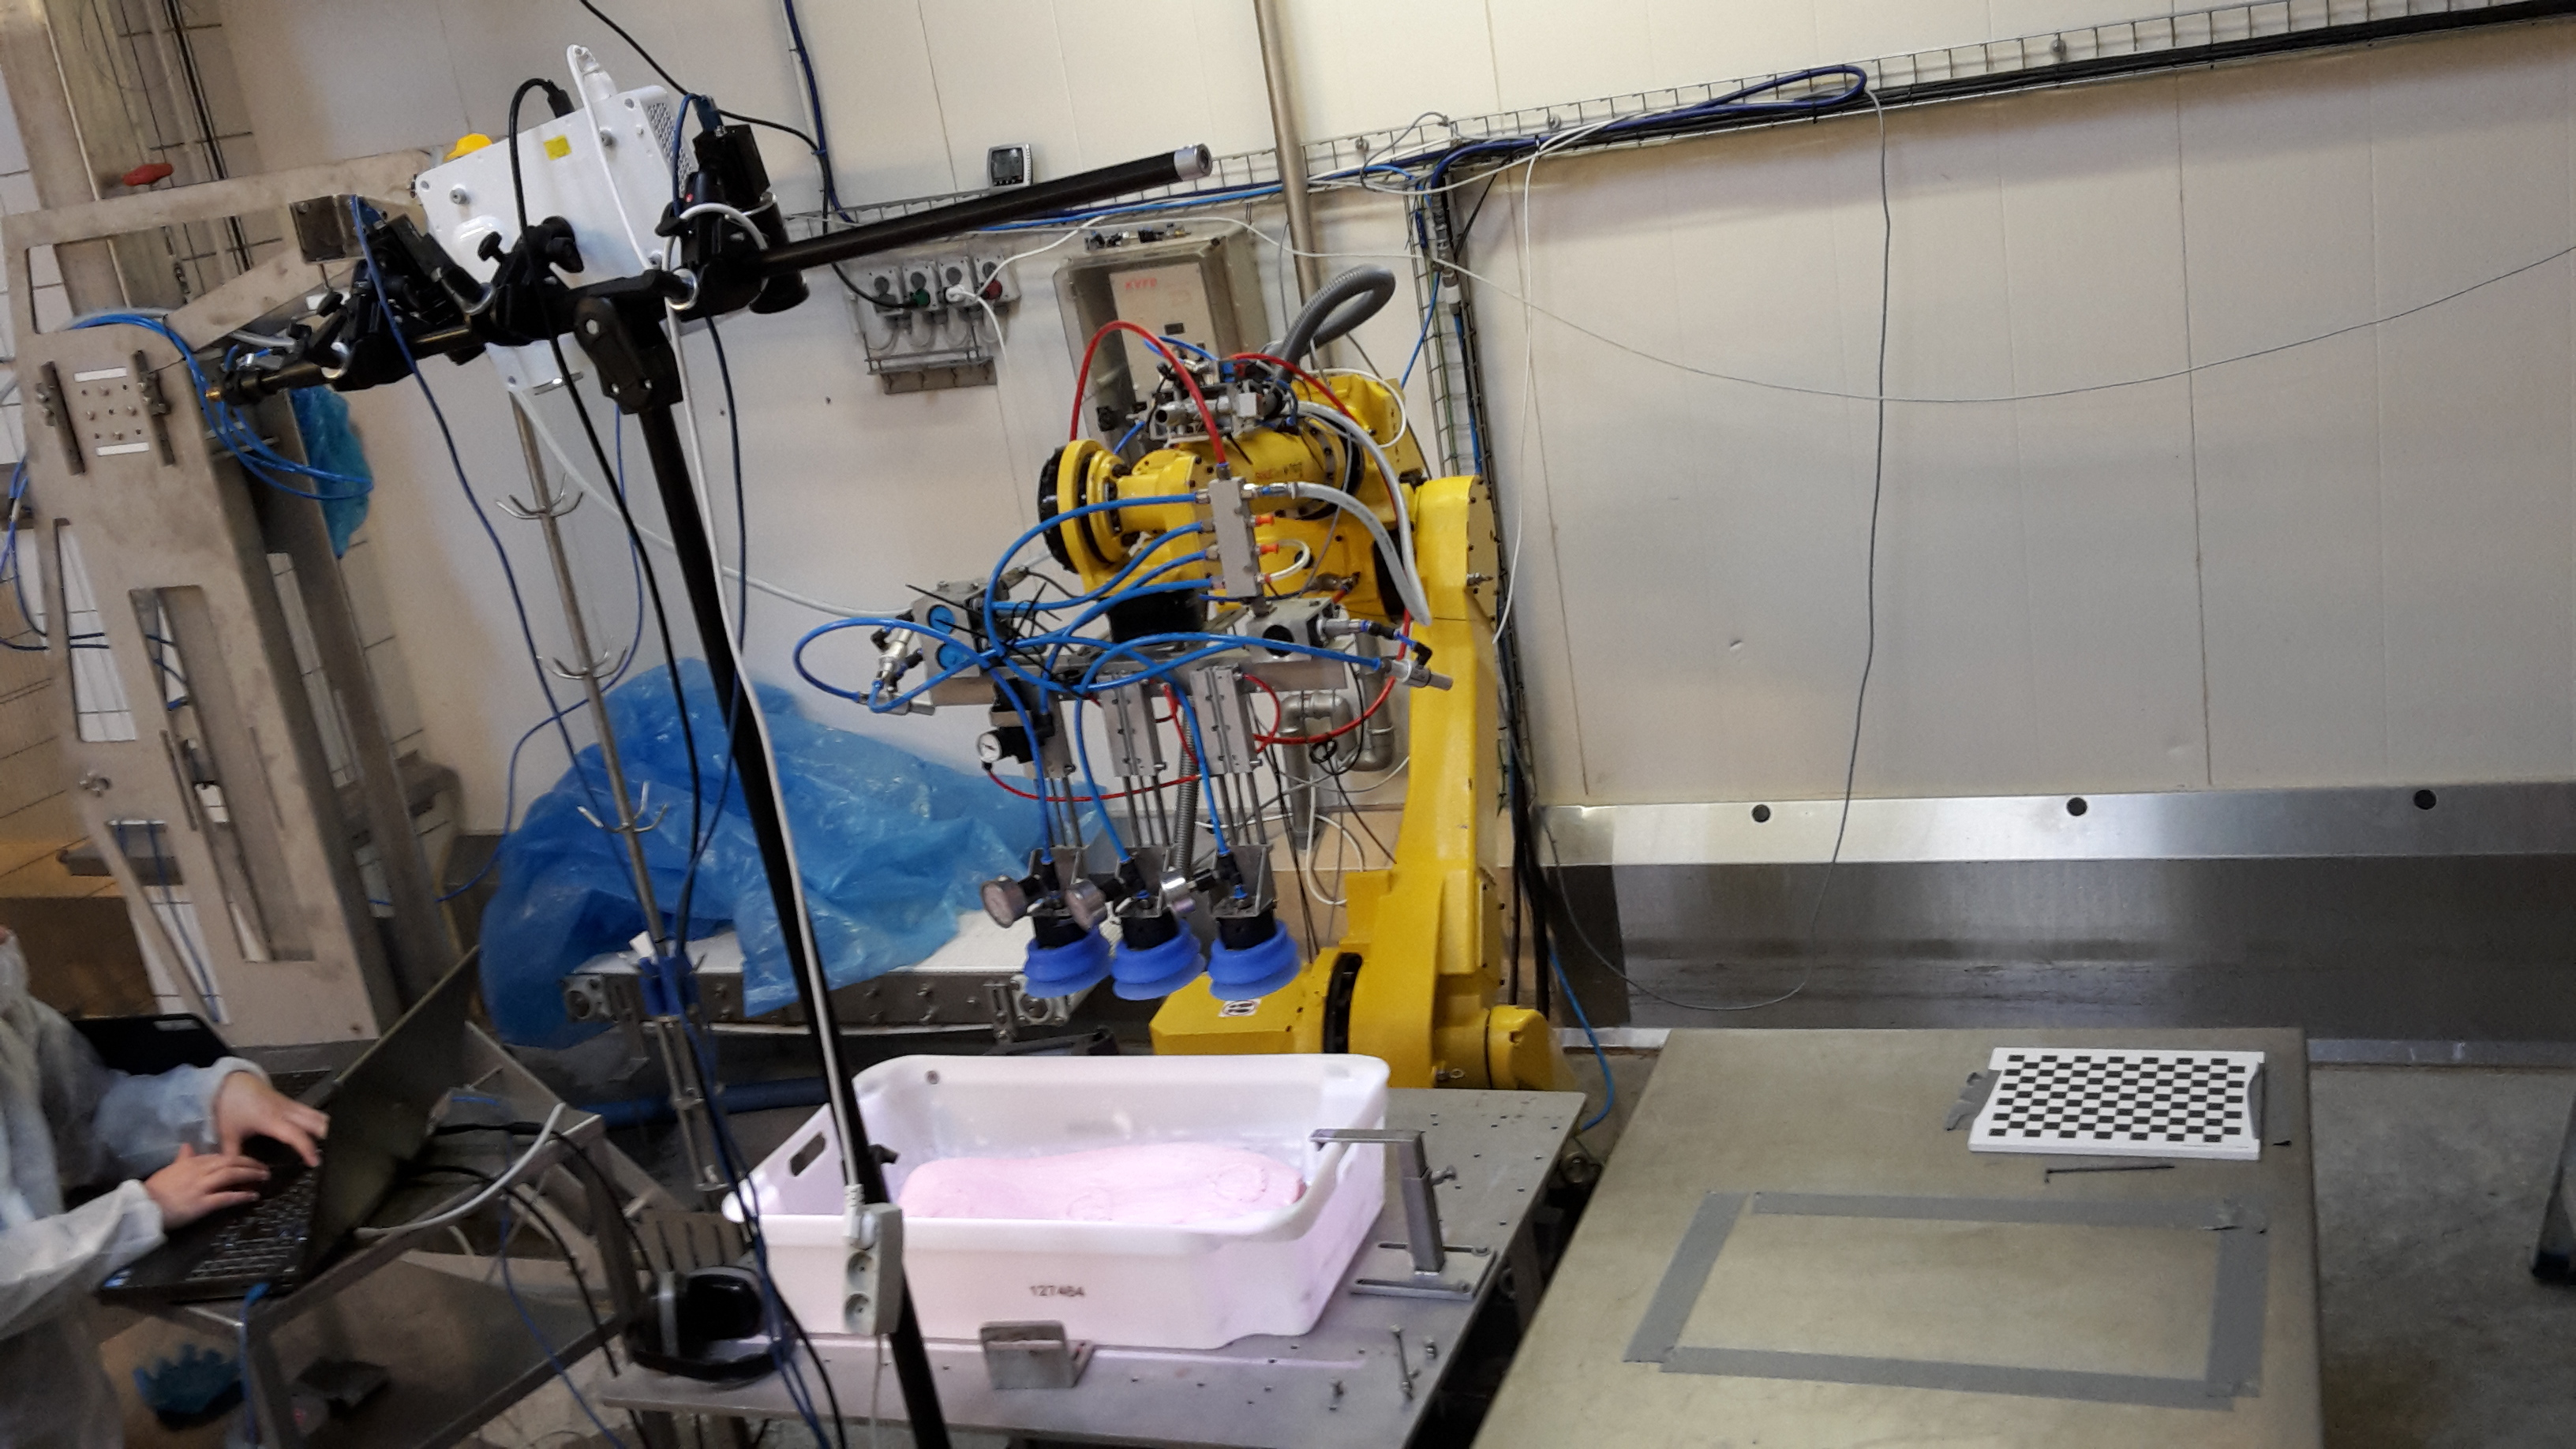
\includegraphics[height=0.65\textheight]{figures/dc_robot}
  \end{figure}
}

\frame{
  \frametitle{Guidance using Structured Light Scanning}
  \begin{figure}
    \centering
    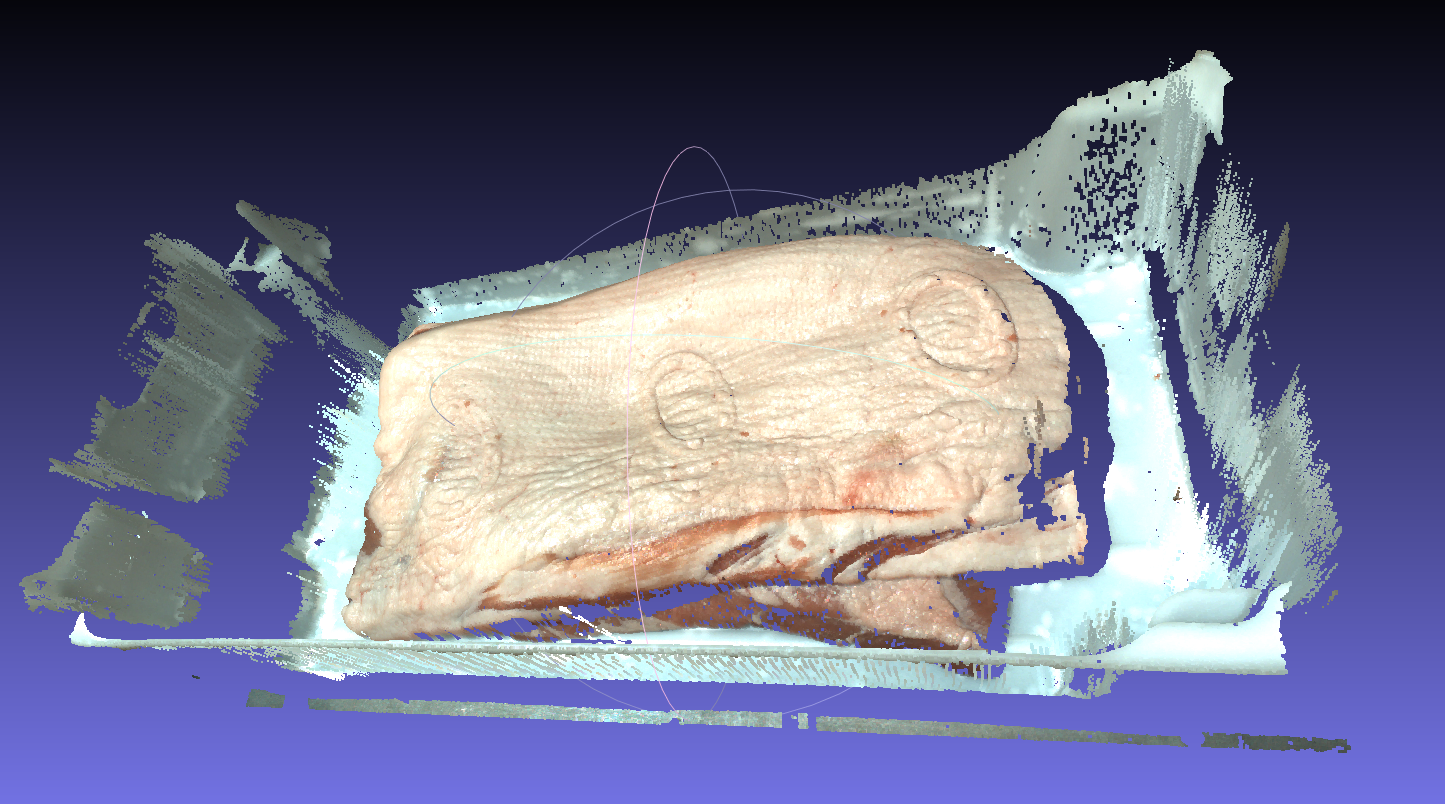
\includegraphics[height=0.6\textheight]{figures/dc_cloud}
    \hfill
    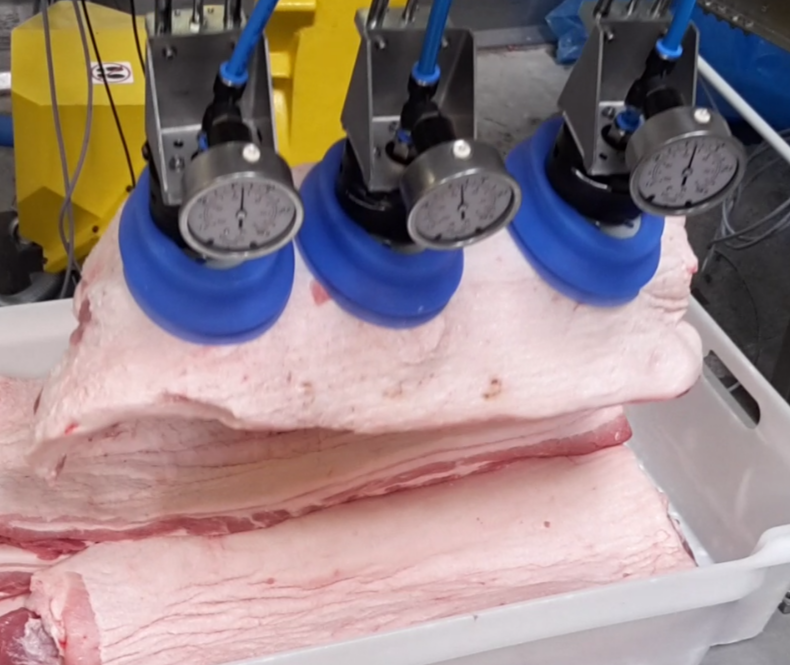
\includegraphics[height=0.6\textheight]{figures/dc_lift}
  \end{figure}
}

%\frame{
%  \frametitle{Segmentation}
%  \begin{figure}
%    \centering
%    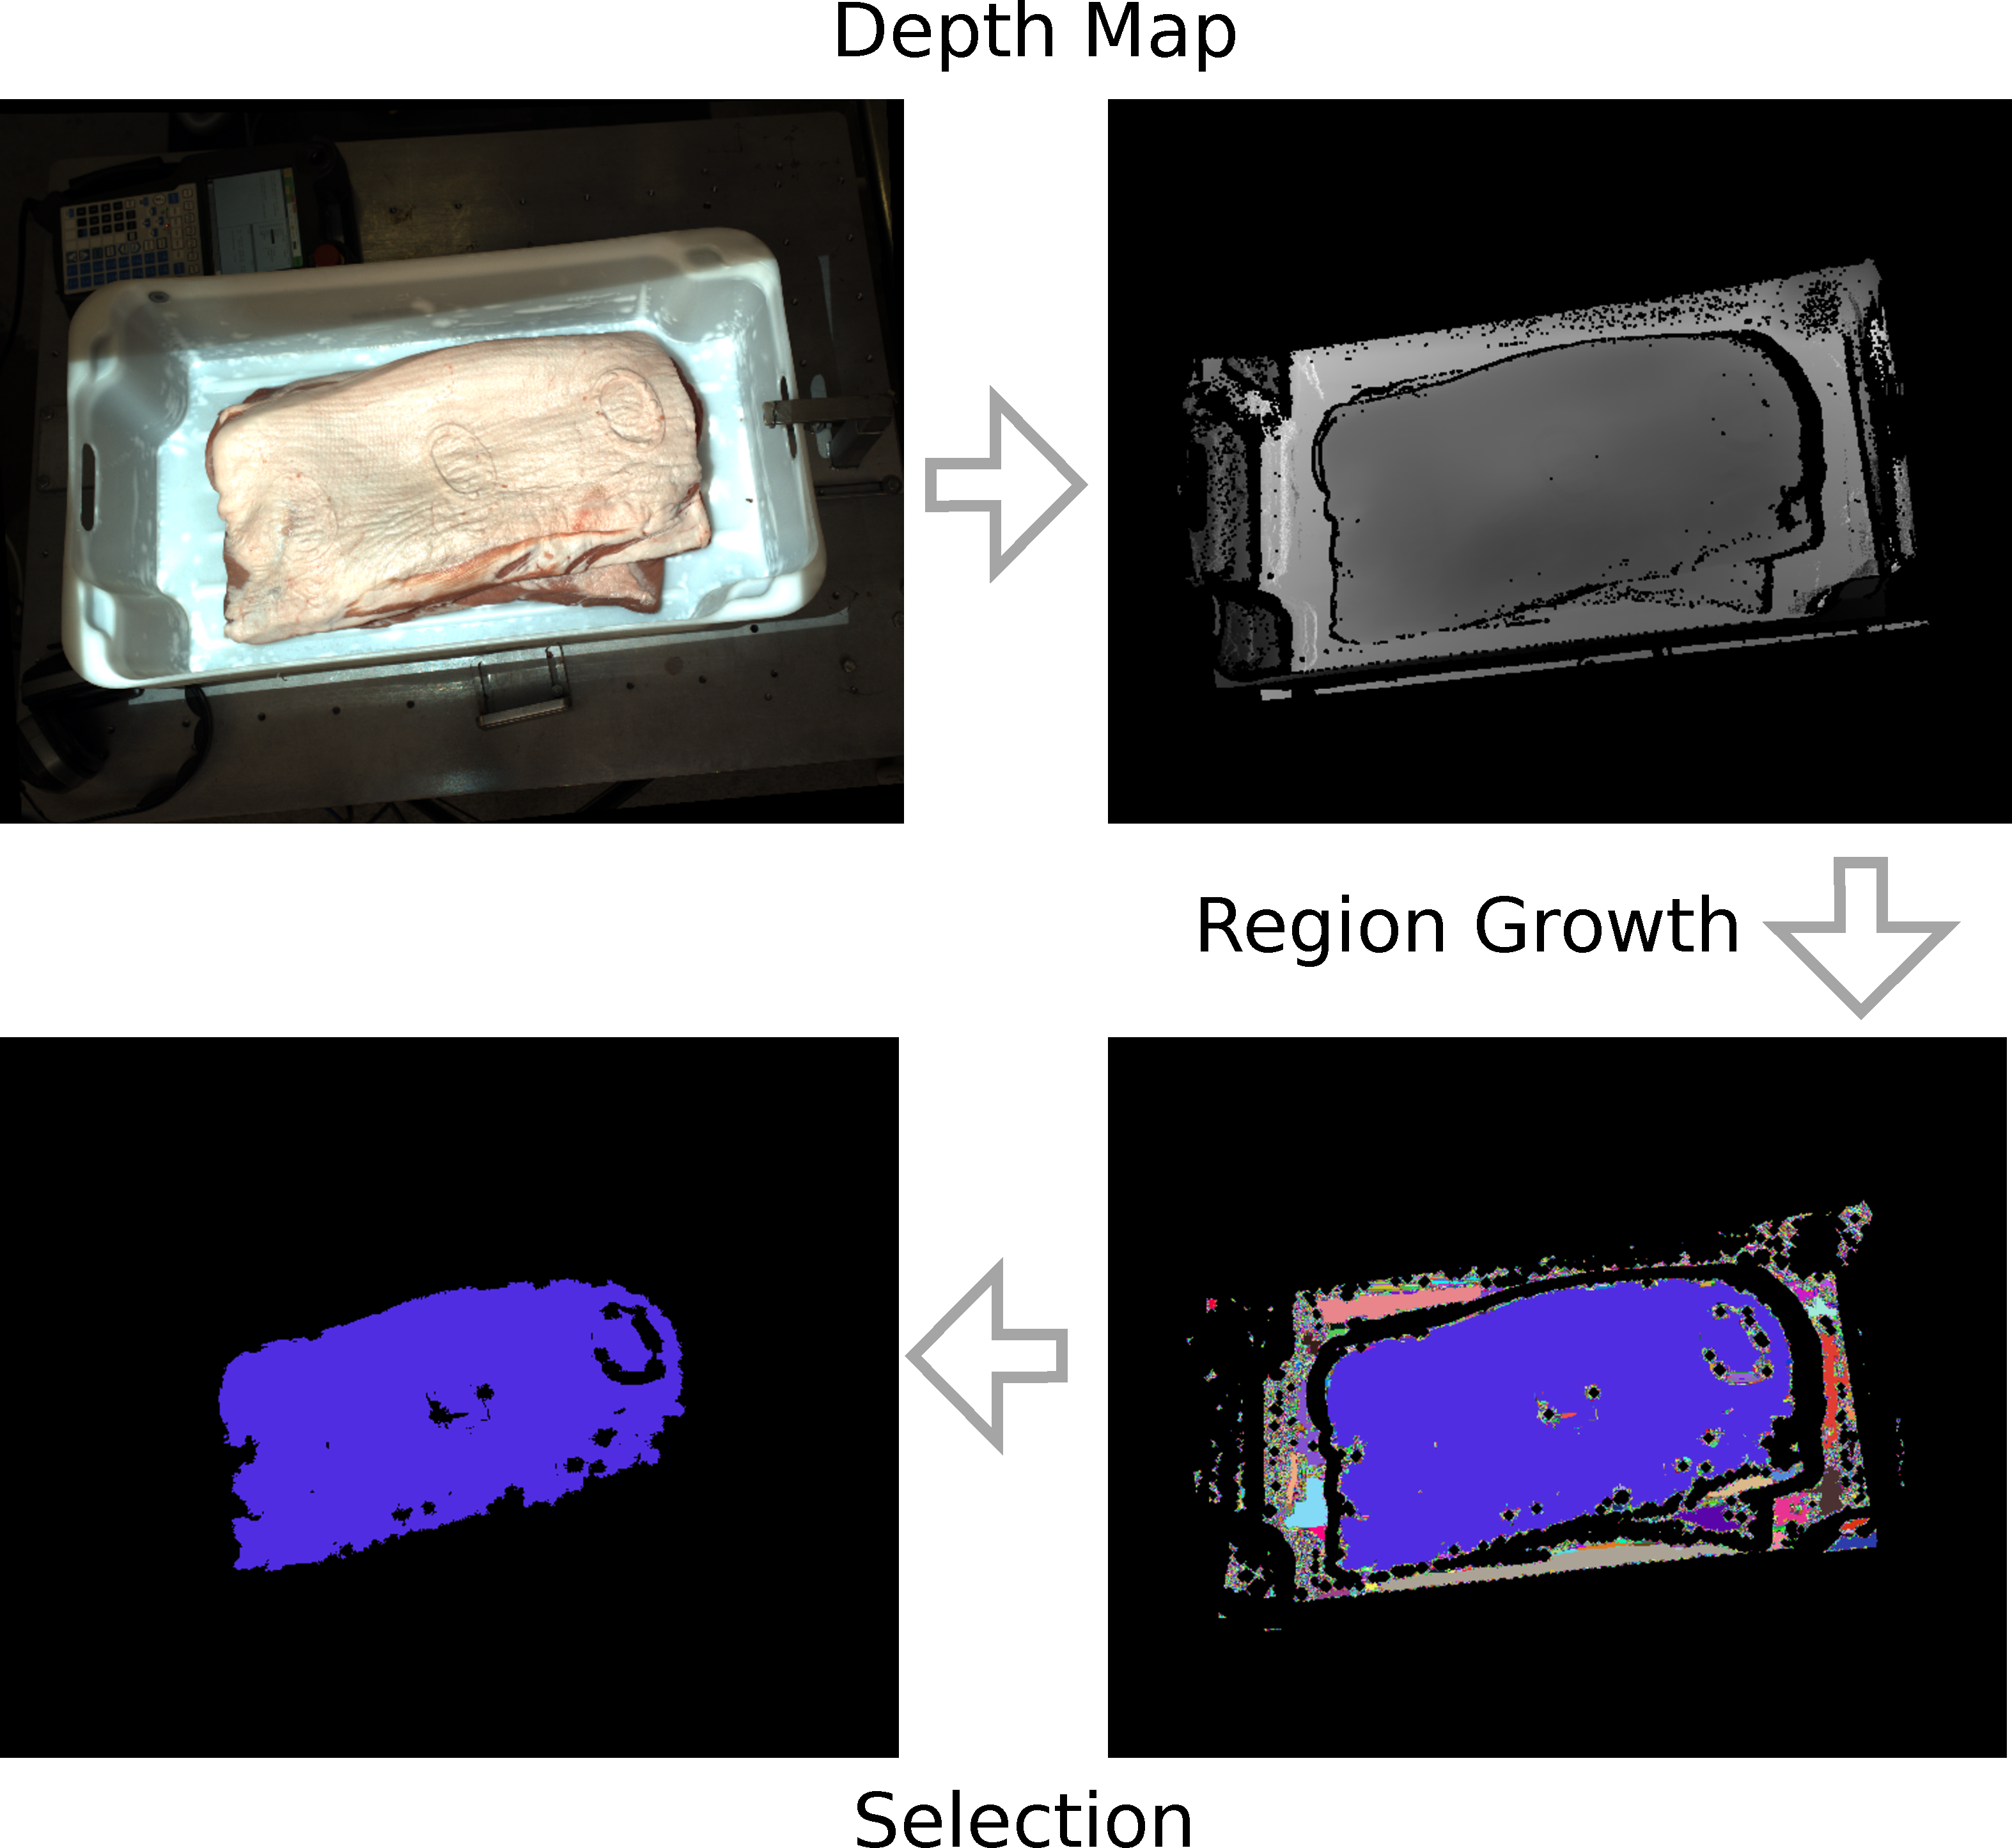
\includegraphics[height=0.9\textheight]{figures/dc_seg}
%  \end{figure}
%}

\frame{
  \frametitle{Demonstration}
  \setlength{\dcwidth}{720px}
  \setlength{\dcheight}{480px}
  \begin{center}
    %\movie[showcontrols, width = 1.35\textheight, height = 0.9\textheight, poster]{}{videos/succesDCManip.avi}
    \href{run:videos/succesDCManip.avi?autostart&loop}{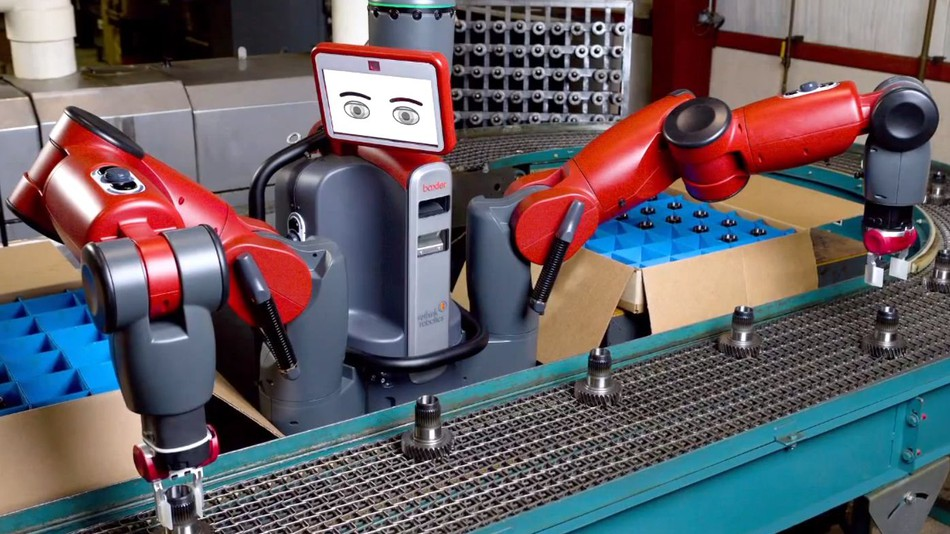
\includegraphics[width=0.4\dcwidth, height=0.4\dcheight]{figures/baxter.jpg}}
  \end{center}
}

\frame{
  \frametitle{Conclusion}
  \begin{itemize}
    \item Pick and place with deformable objects.
    \item Guidance using structured light.
    \item Working prototype demonstrated at Danish Crown, Ringsted.
  \end{itemize}
}
